\documentclass[8pt]{article}  % Adjusts the main text font size
\usepackage{paperlighter}
\usepackage[font=small,labelfont=bf]{caption}
% Recommended, but optional, packages for figures and better typesetting:
\usepackage{microtype}
\usepackage{graphicx}
\usepackage{subfigure}
\usepackage{booktabs} % for professional tables
    
    % Attempt to make hyperref and algorithmic work together better:
    \newcommand{\theHalgorithm}{\arabic{algorithm}}
    
    
    % For theorems and such
    \usepackage{amsmath}
    \usepackage{amssymb}
    \usepackage{mathtools}
    \usepackage{amsthm}
    \usepackage{url}
   
    
    % if you use cleveref..
    \usepackage[capitalize,noabbrev]{cleveref}
    
    %%%%%%%%%%%%%%%%%%%%%%%%%%%%%%%%
    % THEOREMS
    %%%%%%%%%%%%%%%%%%%%%%%%%%%%%%%%
    \theoremstyle{plain}
    \newtheorem{theorem}{Theorem}[section]
    \newtheorem{proposition}[theorem]{Proposition}
    \newtheorem{lemma}[theorem]{Lemma}
    \newtheorem{corollary}[theorem]{Corollary}
    \theoremstyle{definition}
    \newtheorem{definition}[theorem]{Definition}
    \newtheorem{assumption}[theorem]{Assumption}
    \theoremstyle{remark}
    \newtheorem{remark}[theorem]{Remark}
    
    % Todonotes is useful during development; simply uncomment the next line
    %    and comment out the line below the next line to turn off comments
    %\usepackage[disable,textsize=tiny]{todonotes}
    \usepackage[textsize=tiny]{todonotes}
    
    
    \begin{document}
    
    \small\lightertitle{Digital Signal Processing - Laboratory Report 2}
    \begin{flushright}
    \textbf{Nov/2023}
    \lighterauthor{Hongyu Rui, CID:02069033}
    \end{flushright}
    \section{Laboratory 4}

    \begin{minipage}{0.49\textwidth}    
    The Figure \ref{fig:poles} illustrate the zeros and poles of the Moving Average filter (MA)'s system function,
    which is in Z-plane.\\
    The number of poles and zeros increase with increase of filter length.\\
    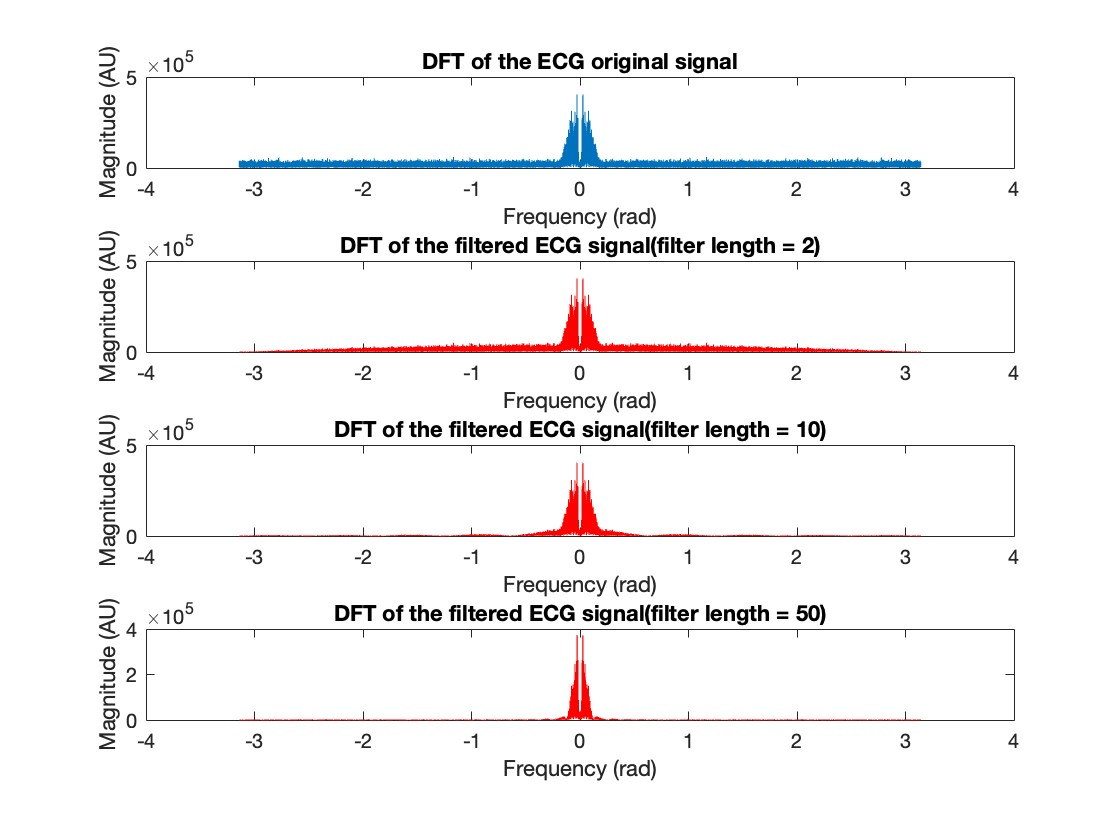
\includegraphics[width=\linewidth]{figure/figure_2.jpg}
    \captionof{figure}{DFT of Original Signal and Effects of Various Filter Lengths}
    \label{fig:ECG_freq}
    \vspace{0.3cm}
    Figure \ref{fig:ECG_time} displays the original ECG signal and its variants filtered at different lengths (2, 10, 50), 
    with their DFTs shown in Figure 1. 
    A notable increase in signal smoothness is observed in the time domain with longer filter lengths. 
    This is attributed to the reduction of high-frequency components, 
    leading to less noise and a smoother appearance in the time-domain signal.
    As for frequency-domain (Figure \ref{fig:ECG_freq}), 
    the filter length increase result in keep ECG frequency and remove noise frequency.
    \end{minipage}
    \hfill
    \begin{minipage}{0.49\textwidth}
    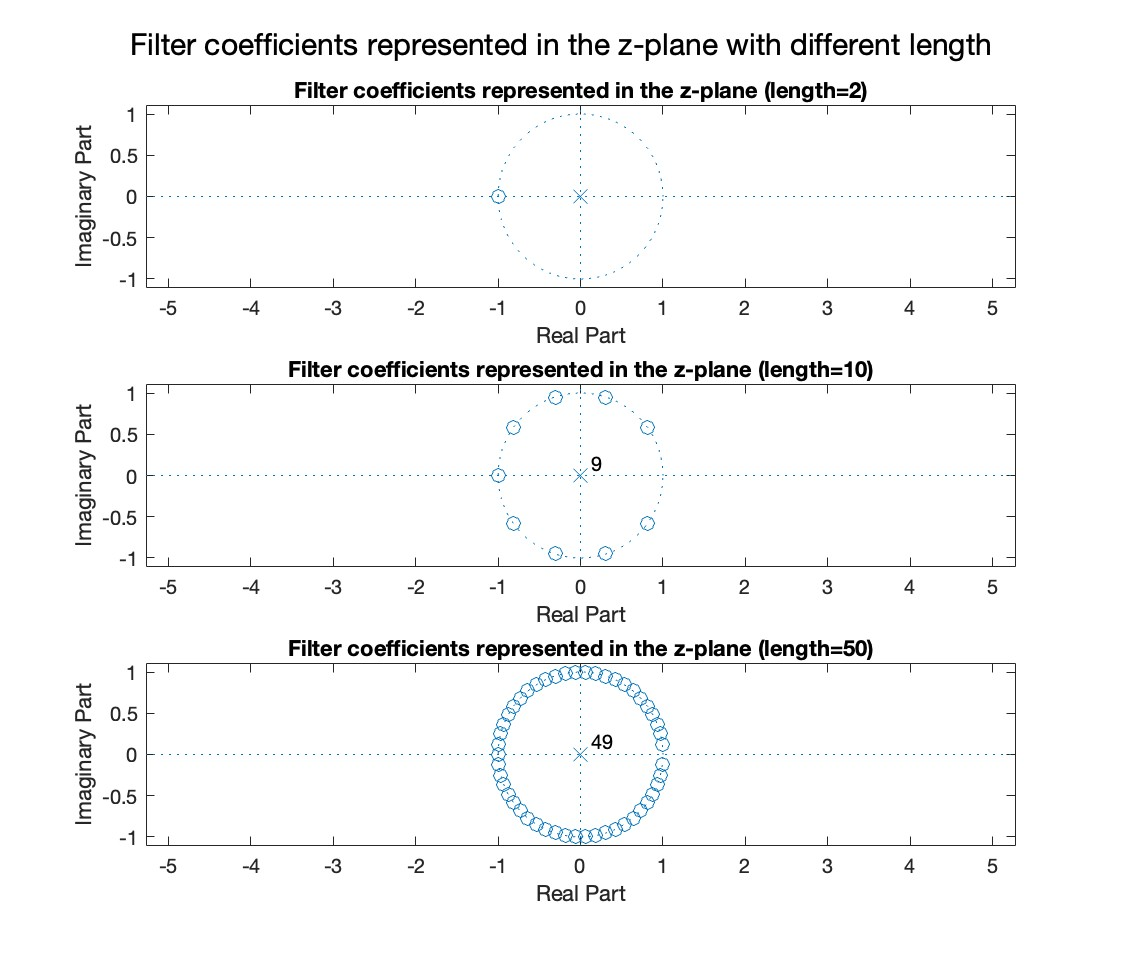
\includegraphics[width=\linewidth]{figure/figure_1.jpg}  
    \captionof{figure}{Zeros and Poles of MA's system function in Z-plane}
    \label{fig:poles}
    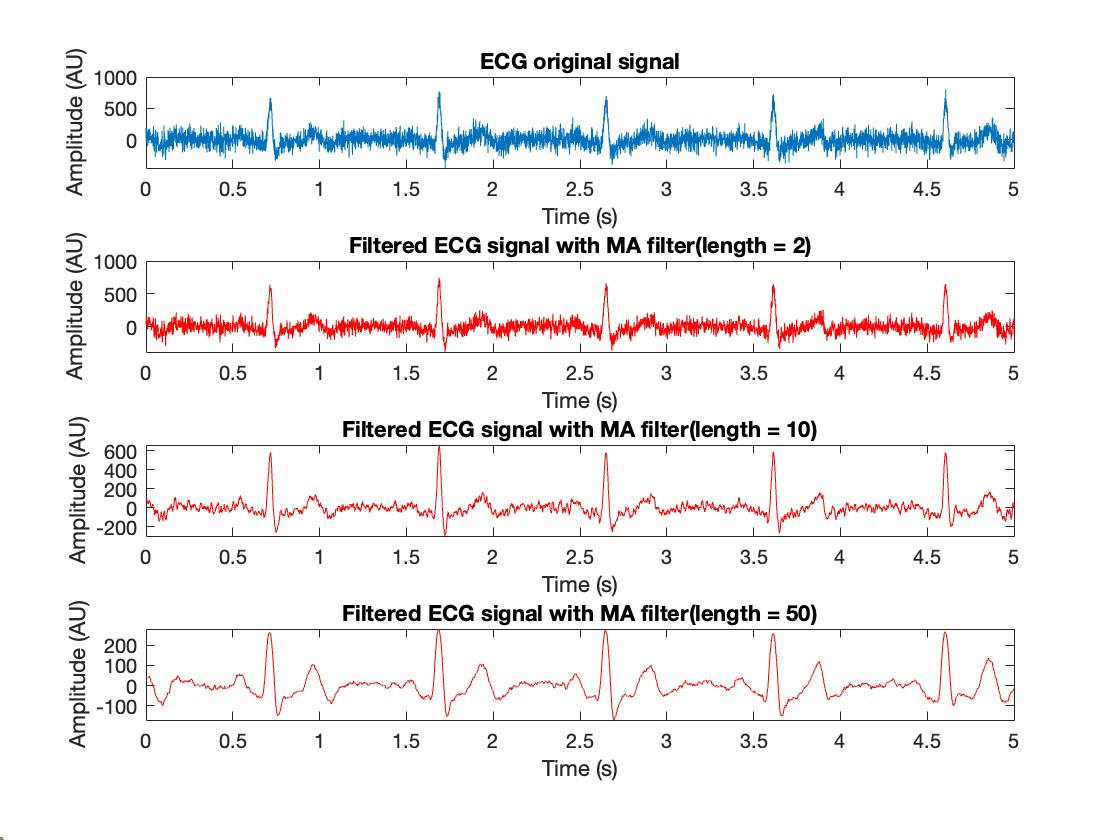
\includegraphics[width=\linewidth]{figure/figure_3.jpg}
    \captionof{figure}{Original ECG Signal and Its Variants Processed with Filters of Varying Lengths}
    \label{fig:ECG_time}
    \end{minipage}


    
    \newpage
    \section{Laboratory 5}
    \begin{minipage}{0.49\textwidth}
         Figure \ref{fig:sinc} illustrates a low pass FIR(Finite Impulse Response) filter,
         specifically a sinc function, in both the time and frequency domains. 
         The cut-off frequency is set at 5Hz, as shown in the frequency domain, 
         with the x-axis units being in Hertz (Hz), not radians.\\

         Figure \ref{fig:MA-filters} and \ref{fig:FIR-filters} display the EMG envelopes obtained using two different types of filters: 
         FIR and MA (Moving Average), 
         each with two filter lengths (400 and 1000). 
         A rectangular window was applied to the FIR filter, 
         and the EMG signal was rectified prior to filtering. 
         Upon comparison, the FIR filter retained more information from the original EMG signal, 
         whereas the MA filter resulted in a more noisy signal. 
         Additionally, an increase in filter length led to a reduction in observed noise for both types of filters.\\
         \vspace{0.3cm}

         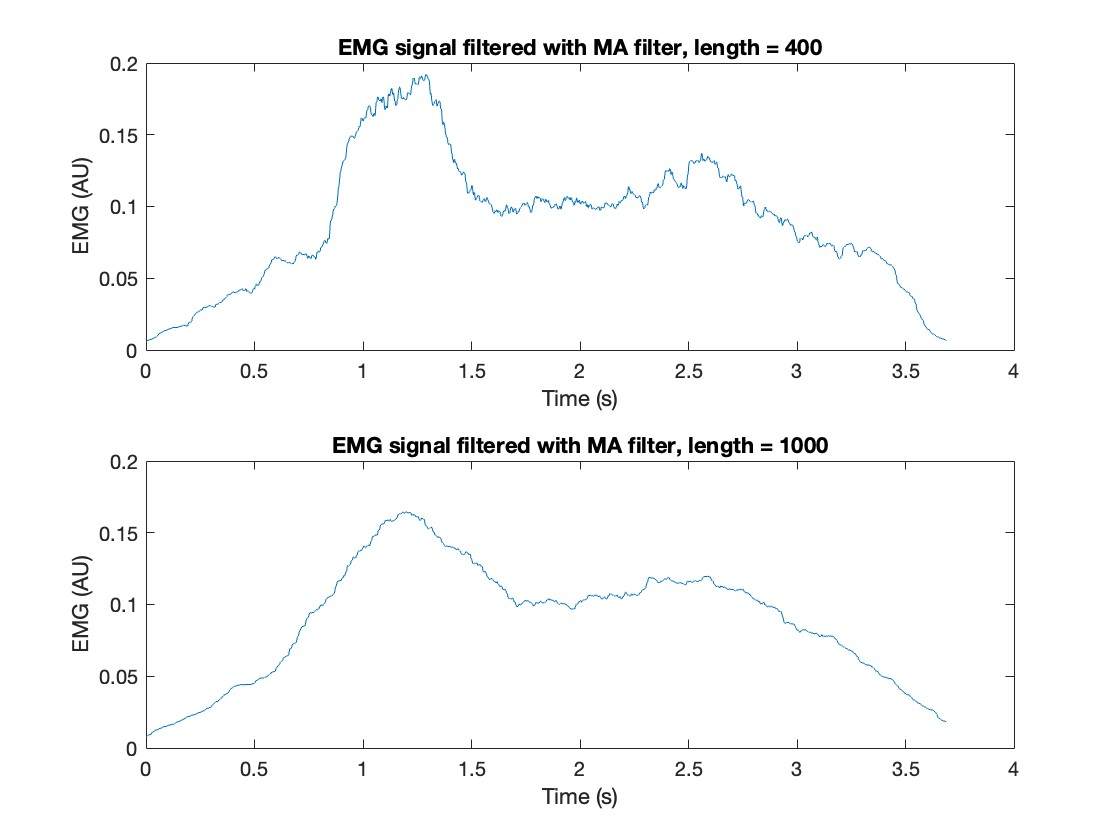
\includegraphics[width=\linewidth]{figure/figure_5.jpg}
         \captionof{figure}{EMG Envelope Processed with MA Filter at Two Different Lengths}
         \label{fig:MA-filters}

         \vspace{0.3cm}
         Figure \ref{fig:window} presents EMG envelopes filtered through a FIR filter with a consistent filter length of 400, 
         using Hanning and rectangular windows. 
         The EMG signal filtered with the Hanning window is noticeably smoother, 
         attributed to the window's bell-shaped curve that gently modulates the signal. 
         In contrast, the rectangular window, 
         with its uniform approach, yields a less smooth envelope.\\

         In the FIR filters, the cut-off frequency remains relatively consistent despite variations in filter length. 
         In contrast, the MA filter exhibits a decrease in cut-off frequency as the window length increases. 
         Regarding FIR filters, an increase in filter length results in an wider truncating window, 
         which leads the impulse response to an longer sinc function, which is more ideal. 
         Additionally, the phase responses for all filters, 
         including both FIR and MA types, 
         are observed to be linear.
         This can be explained by both filters have symmetric impulse response.


    \end{minipage}
    \hfill
    \begin{minipage}{0.49\textwidth}
    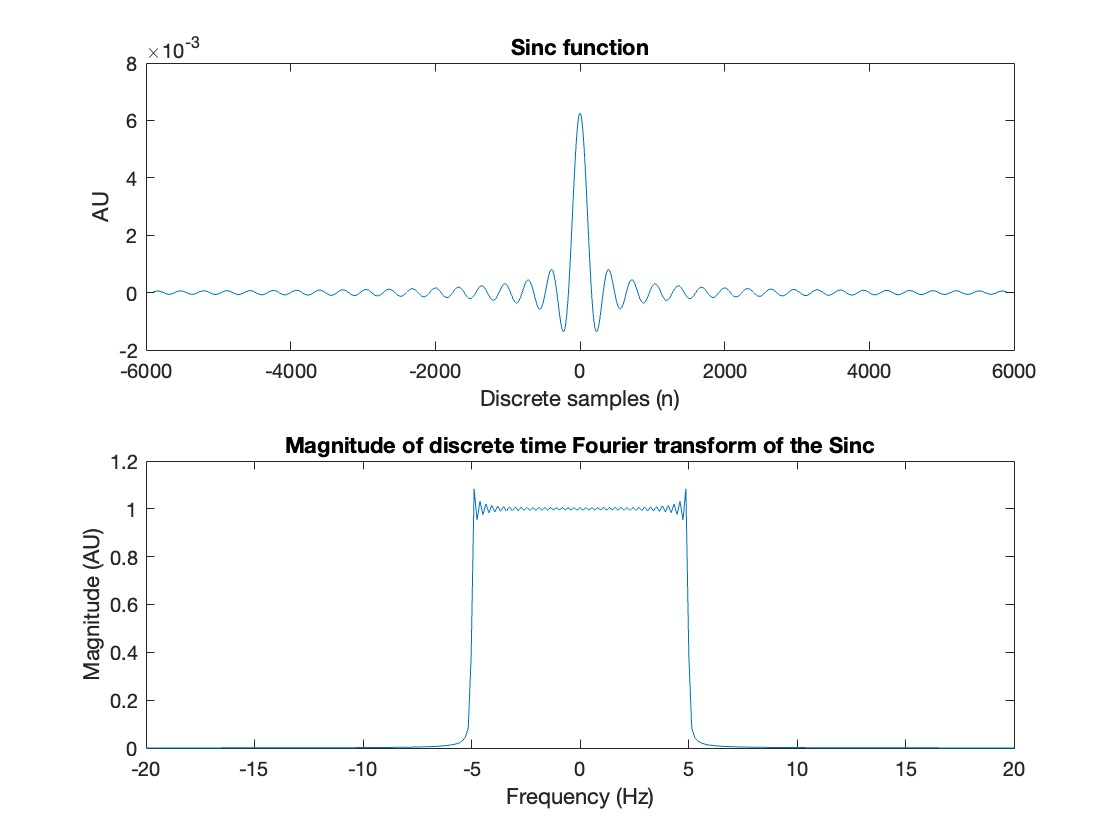
\includegraphics[width=\linewidth]{figure/figure_4.jpg}
    \captionof{figure}{Time and frequency domain of Sinc function}
    \label{fig:sinc}
    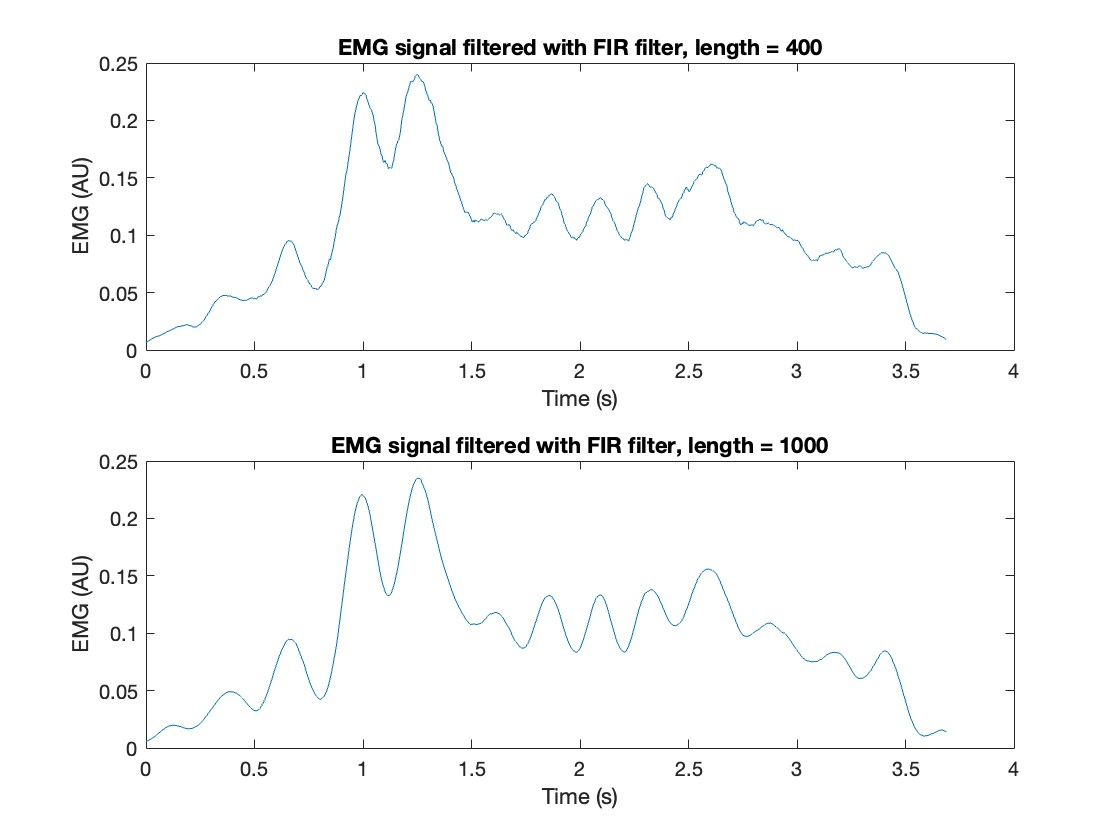
\includegraphics[width=\linewidth]{figure/figure_6.jpg}
    \captionof{figure}{EMG Envelope Processed with FIR Filter at Two Different Lengths}
    \label{fig:FIR-filters}
    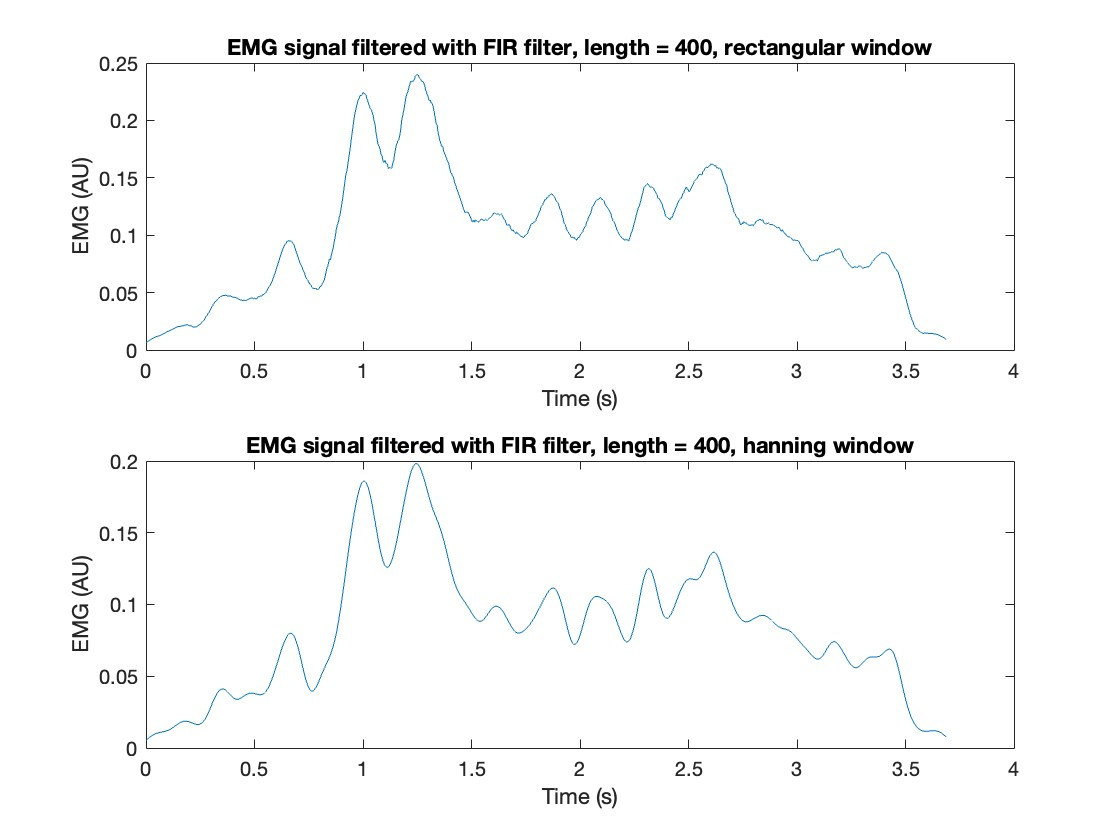
\includegraphics[width=\linewidth]{figure/figure_7.jpg}
    \captionof{figure}{EMG Envelope Processed with FIR Filter at Two Different Lengths}
    \label{fig:window}
    \end{minipage}




    \newpage
    \section{Laboratory 6}
    \begin{minipage}{0.49\textwidth}
        Figure \ref{fig:peaks} displays the frequency spectrum of the EMG signal, 
        where interference peaks at 60 Hz, 120 Hz, and 180 Hz are prominently identified. \\

        \vspace{0.3cm}


        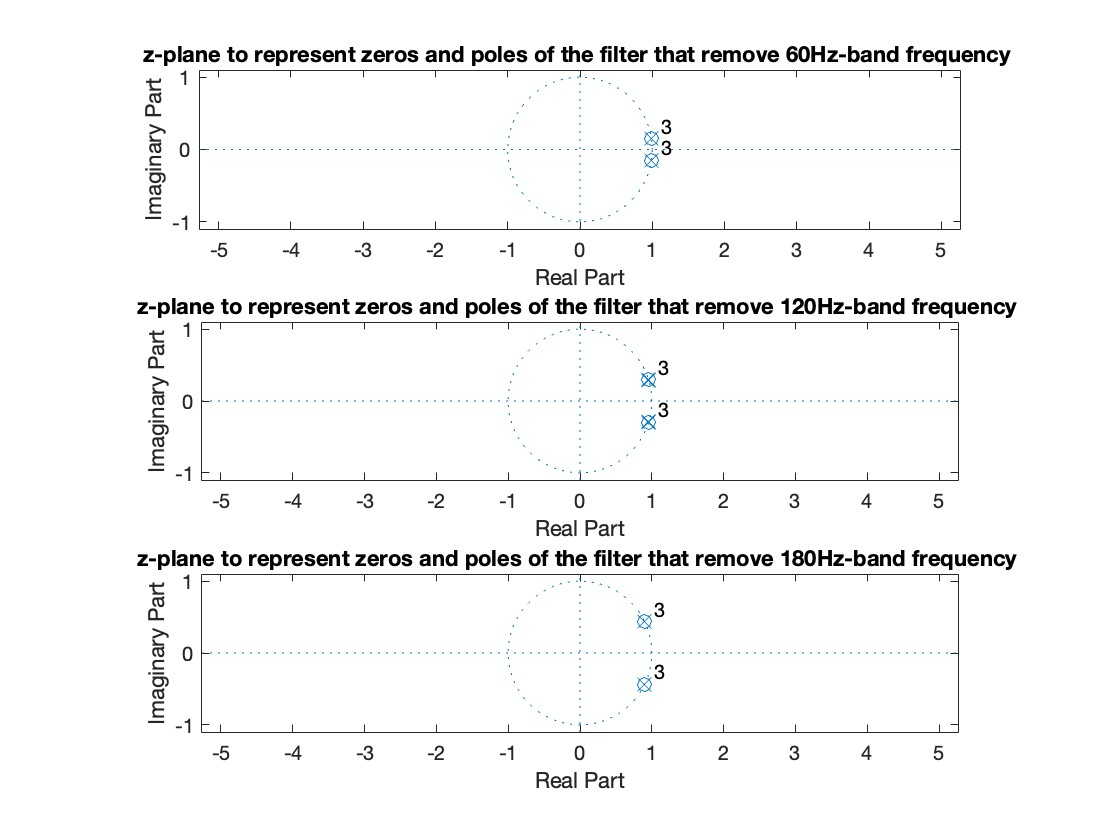
\includegraphics[width=\linewidth]{figure/figure_9.jpg}
        \captionof{figure}{Z-plane for different filters}
        \label{fig:z_plane}

        \vspace{0.3cm}

        Figure \ref{fig:cascade} illustrates the Discrete Fourier Transform of a signal processed through various filters. 
        The original spectrum of the EMG signals is depicted by the red lines, serving as a baseline for comparison. 
        The second plot segment reveals the effect of applying a 60Hz notch filter, which successfully attenuates the 60Hz component. 
        Subsequently, the third segment shows the result of cascading 60Hz and 120Hz filters, 
        and the final segment demonstrates the outcome when all filters—including the 180Hz—are engaged. 
        As indicated, the target frequencies are effectively suppressed by their respective filters.\\
    \end{minipage}
    \hfill
    \begin{minipage}{0.49\textwidth}
        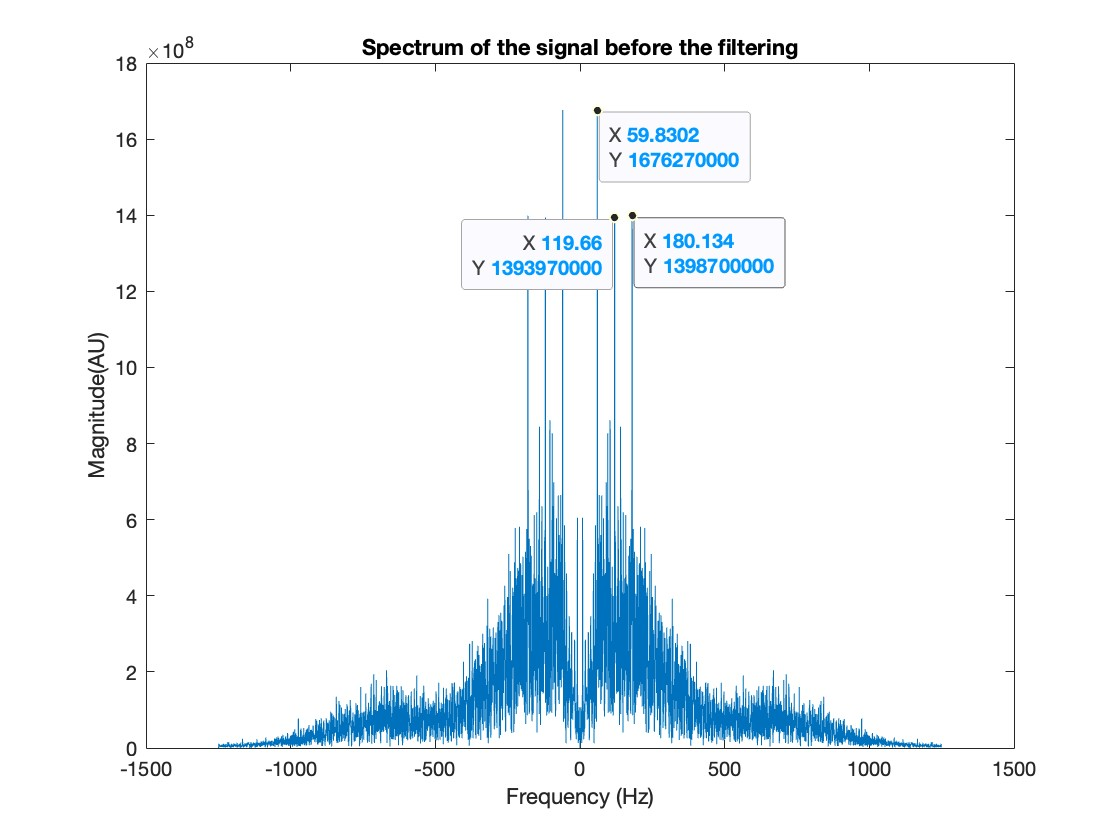
\includegraphics[width=\linewidth]{figure/figure_8.jpg}
        \captionof{figure}{DFT of original EMG signal}
        \label{fig:peaks}

        \vspace{0.3cm}

        In Figure \ref{fig:z_plane}, the poles and zeros for three distinct frequencies are shown. 
        The proximity of poles and zeros can be attributed to the notch filter's design, 
        which combines low-pass and high-pass filters with closely spaced cut-off frequencies.
         Consequently, the poles and zeros of both filter types are closely aligned. 
         Furthermore, an increase in frequency leads to poles more sepzarated, 
         indicating an increase in their imaginary components. 
         Additionally, the nearness of all poles to the unit circle, 
         while not precisely on it, suggests that the filter is marginally stable.

         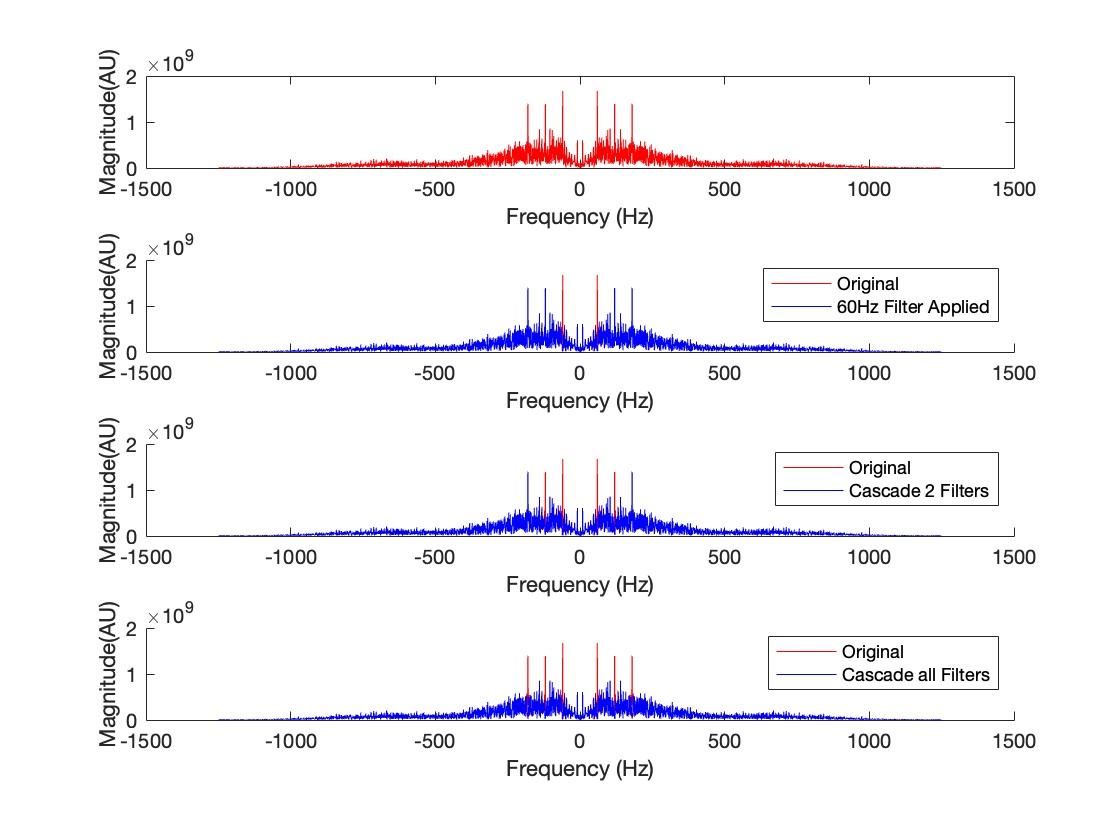
\includegraphics[width=\linewidth]{figure/figure_10.jpg}
         \captionof{figure}{Spectrum Comparison of Original and Filtered Signals}
         \label{fig:cascade} 
    \end{minipage}



    \end{document}